\documentclass[a4paper,11pt]{article}

\usepackage[a4paper, total={6in, 9in}]{geometry}
\usepackage{lmodern} %Latin Modern
\usepackage[hyphens]{url}
\usepackage{biblatex}
\usepackage{amsmath,amssymb}
\usepackage{graphicx}
\usepackage{subcaption}
\bibliography{ref.bib}

\title{Procedural Generation of Strategy RPG Battle Systems -- Interim Report}
\author{Worakarn Isaratham, 140024714}
\begin{document}

\maketitle
	
\section*{Current Progress}

\subsection*{A working initial battle system}

The main artefact of this project is a program that can generate a well-balanced strategy RPG battle system. Currently a simple set of game rules are defined, and an initial battle system within these rules has been implemented, as a starting point for this battle system generator.

The current state of this system has battle generator that creates a random battle environment. The battle is between two parties of equal number of units initially placed on the opposite sides of the battlefield. Each unit has five \textit{basic attributes} (strength, constitution, intelligence, wisdom, and dexterity), and nine more \textit{derived attributes} calculated from some functions over the basic attributes. A unit might wear a weapon and an armour which enhance the wearer's attributes further. The effects of the equipment are also determined from another five \textit{material attributes} (strength, density, plasticity, craftsmanship, and enchantment). 

The game progresses as a series of rounds, on each round each unit get its turn once, with the order determined by the units' speed attribute. A unit can do two things on its turn: (1) move to another cell within its \textit{move range}, and (2) execute one of the following actions: physical attack(short-ranged or long-ranged depending on the weapons), magical attack (Black magic), or magical healing (White magic). A unit hit points is reduced when being attacked, increased when healed, and the unit is removed from the battle once its hit points reaches 0. The game ends when one of the parties have no remaining units on the field. 

The current setup is playable but not very well-balanced, but it has all the quality stated in the primary objectives and some of the secondary objectives:
\begin{itemize}
	\item Difference in tile height affecting the ranges of move and attack.
	\item Elemental magic affecting effectiveness of magical attacks.
\end{itemize}

\subsection*{AI player}

The evaluation of battle systems will be done by observing outcomes of an AI player playing against itself. Such an AI player has been implemented. It is based on the concept of potential field, derived from effects of different actions on total hit-points. 

The potential of a cell is calculated from:
\begin{itemize}
	\item $p_1$: The expected positive outcome to the battle, meaning the highest damage potential to one of the enemy units, or the highest healing potential to one of the friendly units, whichever is higher.
	\item $p_2$: The sum of expected healing potential from all friendly units.
	\item $p_3$: The sum of expected damage potential from all enemy units.
\end{itemize}
The weighted sum $w_1 \cdot p_1 + w_2 \cdot p_2 - w_3 \cdot p_3$ is taken as the potential of the position, with the weights configurable.

Roughly, the AI tries to execute the action that maximizes the expected damage it can cause to the opposing party, or the hit points it can recover to its own party. It also tries to move the unit to the most advantageous position. All of these are based on the maximizing the cell potentials.

From observing the AI playing against itself, this strategy works reasonably well. However it remains to be seen if it will still work in different battle systems.

\subsection*{Graphical user interface}

A graphical user interface that allows a human player to play the game against each other, or against the AI, or watch the AI plays against itself, has been developed. The perspective of the battlefield is rectangular, not the isometric view often used in this game genre. See the screenshots in figure \ref{ss}, and also the attached program \texttt{SRPG.jar}.

\begin{figure}[H!]
	\centering
	\begin{subfigure}{.5\textwidth}
		\centering
		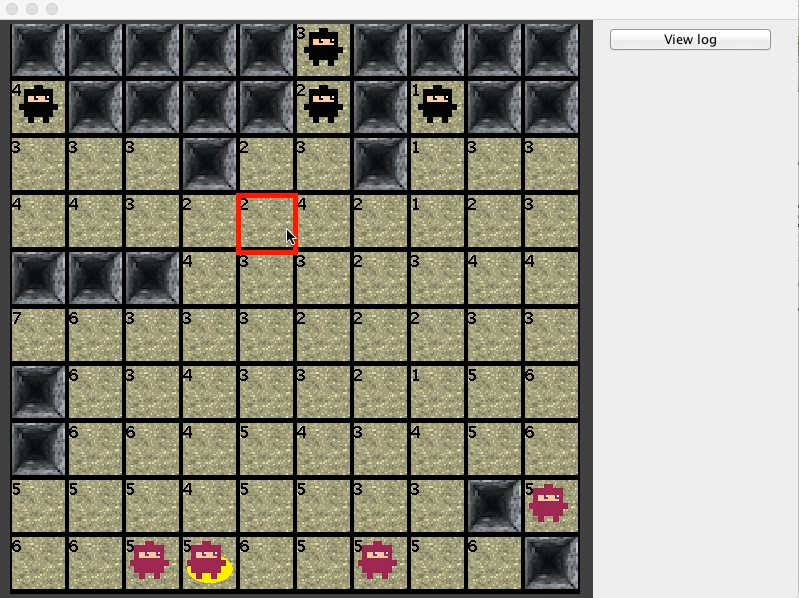
\includegraphics[width=.9\linewidth]{figures/battle0}
		\caption*{The beginning of the battle.}
	\end{subfigure}%
	\begin{subfigure}{.5\textwidth}
		\centering
		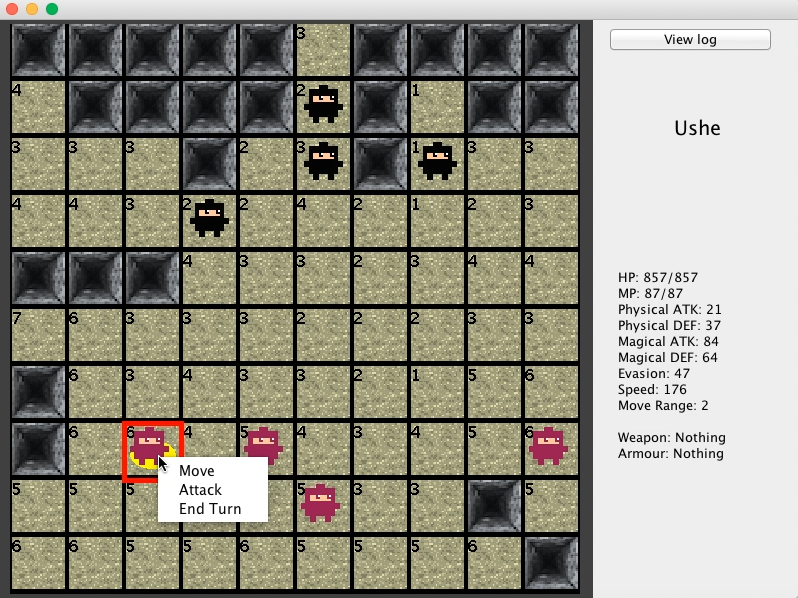
\includegraphics[width=.9\linewidth]{figures/battle4}
		\caption*{List of available commands.}
	\end{subfigure}%
	
	\begin{subfigure}{.5\textwidth}
		\centering
		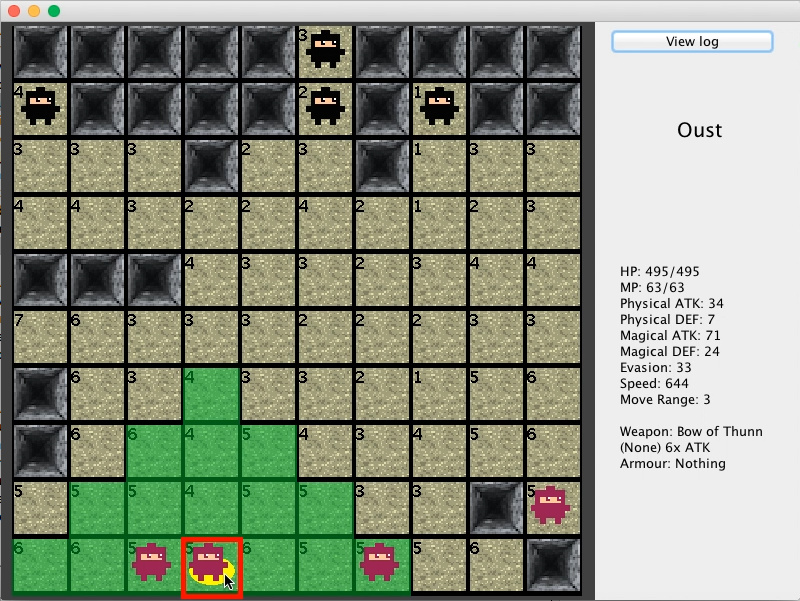
\includegraphics[width=.9\linewidth]{figures/battle5}
		\caption*{Moving range shown in green.}
	\end{subfigure}\begin{subfigure}{.5\textwidth}
		\centering
		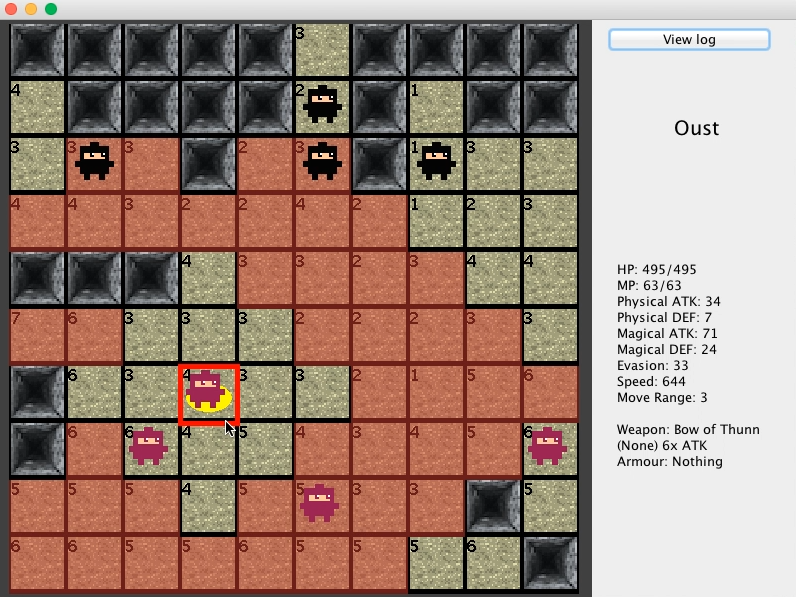
\includegraphics[width=.9\linewidth]{figures/battle1}
		\caption*{Attacking range shown in red.}
	\end{subfigure}
	\begin{subfigure}{.5\textwidth}
		\centering
		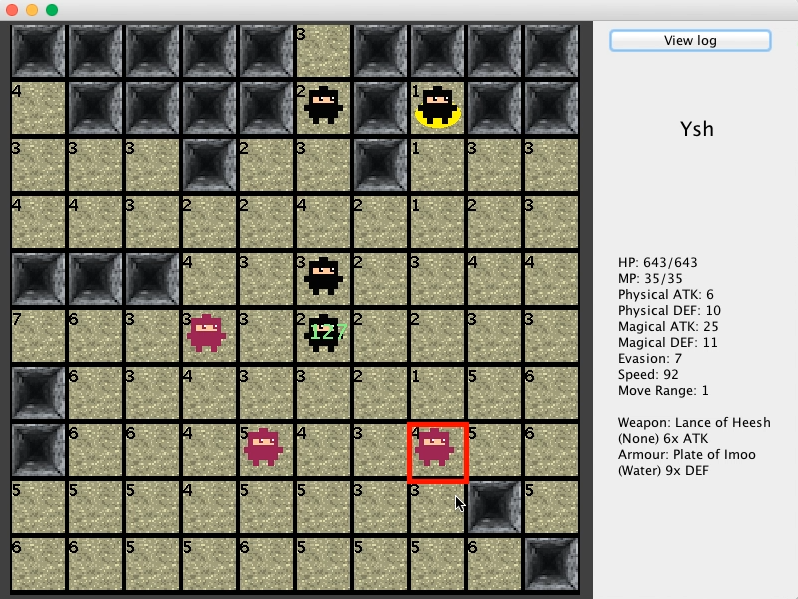
\includegraphics[width=.9\linewidth]{figures/battle2}
		\caption*{The AI heals its unit.}
	\end{subfigure}%
	\begin{subfigure}{.5\textwidth}
		\centering
		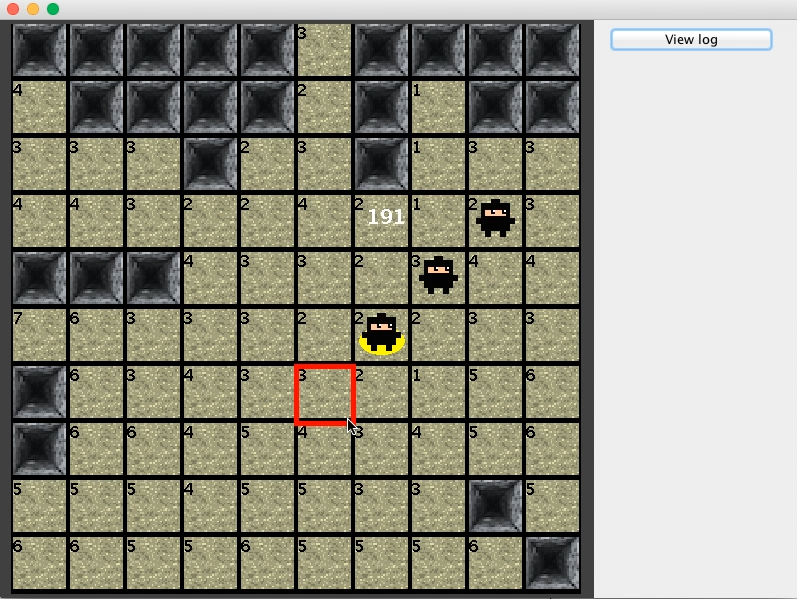
\includegraphics[width=.9\linewidth]{figures/battle3}
		\caption*{Human has lost to AI once again.}
	\end{subfigure}
	\caption{Screenshots of a battle between human player (purple) against the AI (black).}
	\label{ss}
\end{figure}
% some screenshots

\section*{Objectives To Be Accomplished}

\subsection*{Procedural-generation program}

This is the main artefact, and it will be the next major step of this project. The plan is to use evolutionary algorithm to evolve the battle systems to achieve a well-balanced system. This requires the battle system model to be easily parameterized, which has yet to be done. A fitness function is also needed in order to evaluate the quality of battle systems, and it will likely be based on observing the AI playing against itself numerous of times.

\subsection*{Project evaluation}

The battle systems that will be generated by the procedural-generation program need to be manually evaluated that they are indeed well-balanced. An experiment (with humans volunteers) needs to be designed and carried out to accomplish this.

\subsection*{Other secondary enhancements}

There are remaining secondary objectives that might or might not be incorporated into the battle systems, depending on available time. This could be done after the procedural-generation program is completed and before the project evaluation. A consequence is that the AI player will need to be adjusted if any of these objectives are added. These objectives are:
\begin{itemize}
	\item Different terrain types (e.g. lava-filled, water-flooded) that affects the battle.
	\item Support different races and/or jobs for the units, which would boost or limit some certain character attributes.
	\item Support magical spells other than attack and healing e.g. protection, resurrection, status abnormality.
\end{itemize}

\end{document}   
